\documentclass[11pt,border=2pt]{standalone}
\usepackage{amsmath,amssymb}
\usepackage{xcolor}
\usepackage{tikz}
\usepackage{pgfplots}
\pgfplotsset{compat=1.18}
\usetikzlibrary{calc,arrows,positioning,fit,backgrounds,decorations.pathreplacing,patterns}
\definecolor{cElem}{RGB}{40,80,140}
\definecolor{cTrg}{RGB}{190,40,40}
\definecolor{cCell}{RGB}{225,238,248}
\definecolor{cAcc}{RGB}{240,200,120}
\definecolor{cGrey}{RGB}{120,120,120}
\definecolor{cVec}{RGB}{110,55,150}
\begin{document}
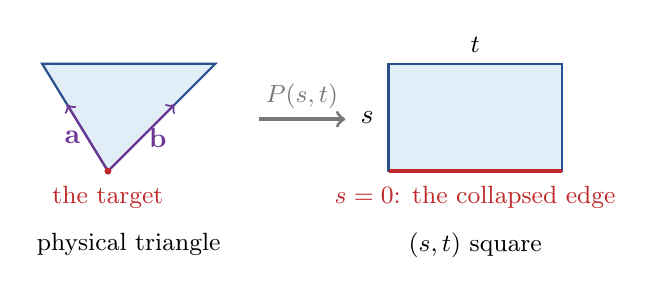
\begin{tikzpicture}[scale=2.2]
  % physical triangle
  \begin{scope}
    \fill[cCell] (0.38,0) -- (0,0.62) -- (1,0.62) -- cycle;
    \draw[cElem,thick] (0.38,0) -- (0,0.62) -- (1,0.62) -- cycle;
    \draw[->,cVec,thick] (0.38,0) -- ($(0.38,0)!0.62!(0,0.62)$) node[midway,left=-1pt] {$\mathbf{a}$};
    \draw[->,cVec,thick] (0.38,0) -- ($(0.38,0)!0.62!(1,0.62)$) node[midway,right=-1pt] {$\mathbf{b}$};
    \fill[cTrg] (0.38,0) circle (0.02);
    \node[cTrg,below,font=\small] at (0.38,-0.03) {the target};
    \node[below,font=\small] at (0.5,-0.30) {physical triangle};
  \end{scope}
  % arrow
  \draw[->,very thick,cGrey] (1.25,0.3) -- (1.75,0.3) node[midway,above] {\small $P(s,t)$};
  % (s,t) square
  \begin{scope}[xshift=2cm]
    \fill[cCell] (0,0) rectangle (1,0.62);
    \draw[cElem,thick] (0,0) rectangle (1,0.62);
    \draw[cTrg,ultra thick] (0,0) -- (1,0);
    \node[cTrg,below,font=\small] at (0.5,-0.03) {$s=0$: the collapsed edge};
    \node[left] at (-0.03,0.31) {$s$};
    \node[below,font=\small] at (0.5,-0.30) {$(s,t)$ square};
    \node[above,font=\small] at (0.5,0.63) {$t$};
  \end{scope}
\end{tikzpicture}
\end{document}
